
\begin{figure}[t!]
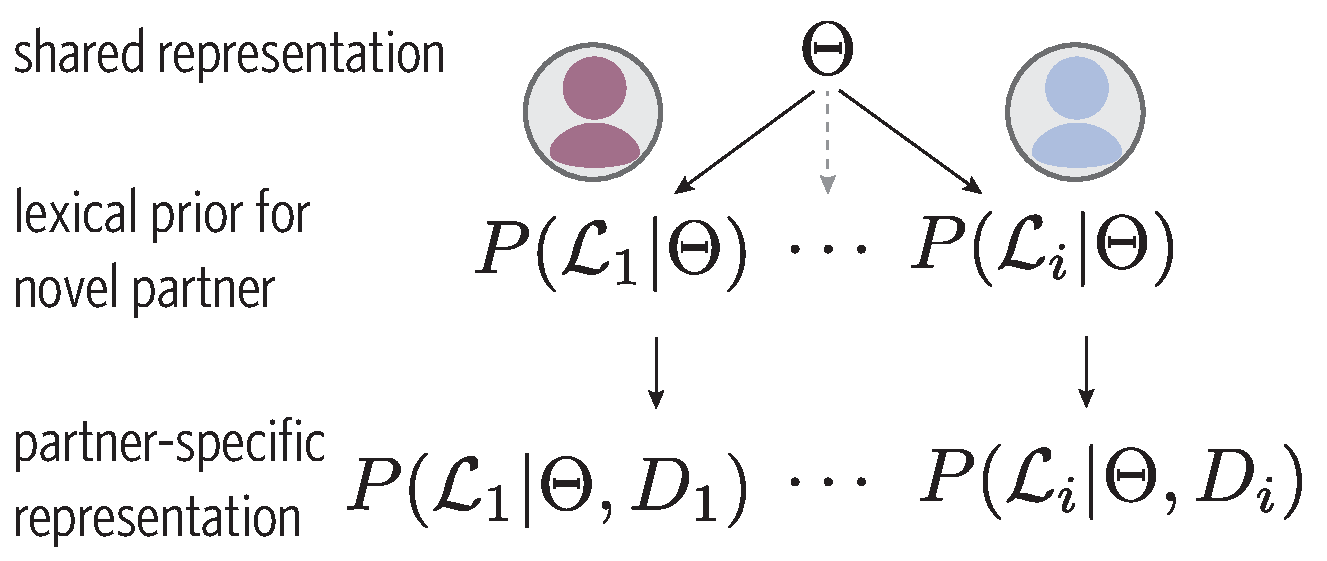
\includegraphics[scale=0.4]{./figures/task1_model.pdf}
\caption{Schematic of hierarchical Bayesian model.}
\label{fig:model_schematic}
\end{figure}

In this section, we provide an explicit computational account of the cognitive mechanisms supporting the balance between community-level stability and partner-specific flexibility.
%Our model is based on three basic principles: 
%
%\begin{enumerate}
%\item \emph{lexical uncertainty}: beliefs about the underlying conventions used by other agents are represented and updated probabilistically \cite{bergen_pragmatic_2016}
%\item \emph{pragmatic reasoning}: agents expect other agents to use language in a cooperative manner, and do so themselves  \cite{GoodmanFrank16_RSATiCS}
%\item \emph{inductive learning}: agents expect their social world to be structured, such that common beliefs may be shared even by individuals they have never met \cite{}
%\end{enumerate}
%We formalize the mechanisms of uncertainty, adaptation, and generalization in a hierarchical Bayesian model.
We begin with the assumption of \emph{lexical uncertainty} \cite{smith_learning_2013,bergen_pragmatic_2016}. 
Instead of assuming meanings are shared in common ground, we assume each agent has uncertainty over the exact meaning of words to their partner.
Critically, in a hierarchical model, this uncertainty is represented by a multi-level prior. 
At the highest level of the hierarchy is \emph{community-level} uncertainty $P(\Theta)$, where $\Theta$ represents an abstract ``overhypothesis" about the overall distribution of possible partners. 
$\Theta$ then parameterizes the agent's \emph{partner-specific} uncertainty $P(\phi_{k} | \Theta)$, where $\phi_k$ represents the specific system of meaning used by partner $k$ (see Fig. \ref{fig:model_schematic}). 

Given observations $D_k$ from interactions with partner $k$, the agent updates their beliefs about the latent system of meaning using Bayes rule:
\begin{equation}
\begin{array}{rcl}
\label{eq:joint_inference}
P(\phi_k, \Theta | D_k)  & \propto &  P(D_k | \phi_k, \Theta) P(\phi_k, \Theta) \\
                           & =   & P(D_k | \phi_k) P(\phi_k | \Theta) P(\Theta)
\end{array}
\end{equation}
This joint inference decomposes the learning problem into two terms, a prior term $P(\phi_k | \Theta)P(\Theta)$ and a likelihood term $P(D_k | \phi_k)$.
The prior captures the idea that different partners may share aspects of meaning in common.
In the absence of strong evidence that partner-specific language use departs from this common structure, the agent ought to regularize toward background knowledge of the population's conventions.
The likelihood represents predictions about how a partner using a particular system of meaning will use language in context.

This joint posterior over meanings has two consequences for convention formation.
First, it allows agents to maintain partner-specific expectations $\phi_k$ by marginalizing over community-level uncertainty:
\begin{equation}
P(\phi_k | D_k) = \int_{\Theta}P(D_k | \phi_k) P(\phi_k | \Theta) P(\Theta)  d\Theta
\end{equation}
Second, the hierarchical structure provides an inductive pathway for data to inform beliefs about community-wide conventions.
Agents update their beliefs about $\Theta$ by marginalizing over data accumulated from different partners:
\begin{equation}
P(\Theta | D) = P(\Theta) \int_{\phi} P(D_k | \phi_k) P(\phi_k | \Theta) d\phi
\end{equation}
where $D = \bigcup_{k=1}^N D_k$, $\phi = \phi_1 \times \dots \times \phi_N$, and $N$ is the number of partners previous encountered. 
After multiple partners are inferred to have a similar system of meaning, beliefs about $\Theta$ shift to represent this abstracted knowledge: it becomes more likely that a novel partner will share it as well.
This transfer is sometimes referred to as ``sharing of strength'' or ``partial pooling'' because pooled data is smoothly integrated with domain-specific knowledge.

The principle of \textit{pragmatic reasoning} plays two distinct roles in our model.
First, when an agent is inferring their partner's latent representation of meaning from their observable behavior (Eq.~\ref{eq:joint_inference}), we assume that the likelihood reflects Gricean principles.
In other words, the agent assumes their partner is using language in a cooperative manner.
Second, agents do not only make passive inferences from data, they actually \emph{use language} in interaction, given their current beliefs.
We assume that production and comprehension is also guided by Gricean principles.

%In this reference game setting, we can explicitly specify the likelihood and prior terms in Eq. (1). 
More specifically, we draw upon the recent Rational Speech Act (RSA) framework, which formalizes the Gricean assumption of cooperativity as recursive social inference \cite{frank_predicting_2012,GoodmanFrank16_RSATiCS,FrankeJager16_ProbabilisticPragmatics}.~A pragmatic speaker denoted by $S_1$ attempts to trade off informativity to an imagined listener against the cost of producing an utterance, while a pragmatic listener $L_1$ inverts their generative model of a speaker to infer the intended target.
This chain of recursive reasoning grounds out in a \emph{literal listener} $L_0$, who identifies the intended target directly using a softmax over the parameterized lexical meaning function $\mathcal{L}_{\phi_k}$.
For any utterance $u$ and world state $o$, the function $\mathcal{L}$ function returns the extent to which $u$ applies to $o$.\footnote{While this function is traditionally a binary truth-conditional variable, $\mathcal{L}_{\phi_k}: (u,o) \rightarrow \{0,1\}$, recent work has also argued for a continuous semantics mapping to the full real interval $[0,1]$  \cite{degen2020redundancy}}

This model can be specified as follows:
\begin{align}
L_0(o | u, \phi_k) &\propto  \mathcal{L}_{\phi_k}(u,o)\hfill\label{eq:RSA}\\
S_1(u | o, \phi_k) &\propto   \exp\{w_S \log L_0(o | u, \phi_k) - w_C \cdot c(u)\}\nonumber   \\
L_1(o | u, \phi_k) &\propto   \exp\{w_L \log S_1(u | o, \phi_k)\}\nonumber
\end{align}
where $c(u)$ is a function giving the cost of producing $u$; $w_S$ and $w_C$ are free parameters controlling the relative weights of the speaker's informativity and parsimony, respectively; and $w_L$ controls the optimality of the listener.

Under any possible value of $\phi_k$, these functions can be used as a likelihood for observations of language use $P(D_k | \phi_k)$ to infer their partner's lexicon (Eq.~\ref{eq:joint_inference}).
They assign a probability to each word or object that partner $k$ has chosen, assuming that their partner behaved according to Gricean maxims.
In addition to using RSA as a likelihood for inferring $\Theta$ and $\phi_k$, we assume that the agents use these functions to \emph{act} on each trial of their interaction.
We sample from their posterior predictive, marginalizing over the agent's current beliefs about $\phi_k$:
\begin{align}
L(o|u) &\propto   \exp\left\{ \textstyle{\int_{\phi_k}} P(\phi_k | D_k) w_L \log S_1(u|o, \phi_k)d\phi_k\right\}\label{eq:marginalized}\\
S(u|o) &\propto  \exp\left\{ \textstyle{\int_{\phi_k}} P(\phi_k | D_k)  w_S \log L_1(o| u, \phi_k) - w_C c(u)d\phi_k\right\}\nonumber
\end{align}

\subsection{Auxiliary assumptions}

The formulation in the previous section presents the core of our theory.
Here, we highlight several auxiliary assumptions we make for the simulations throughout this paper.

First, what data $D_k$ should each agent use to update their beliefs at a particular point in an interaction?
In our simulations, we allow the same agent to switch between the speaker and listener role, so a partner may produce utterances $u$ on some trials and object choices $o$ on other trials; consequently, we assume an agent always conditions on feedback from their \emph{partner's} choices.
This assumption of symmetry, where each partner equally adjusts to the other, creates a clear coordination problem. 
In the case of an error, where the agent in the listener role hears the utterance $u$ and chooses an object $o'$ other than the intended target $o^*$, they will receive feedback about the correct target and subsequently condition on the likelihood that the speaker chose this utterance to convey this target, $S_1(u | o^*)$. 
Meanwhile, the agent in the speaker will subsequently condition on the likelihood that the listener chose the object $o'$ upon hearing their utterance $L_1(o' | u)$.
In other words, each agent will subsequently condition on slightly different data.
While we consider this assumption to be the most challenging coordination setting, it is also possible to assume that agents in one role (e.g. the listener role) are expected to adapt more strongly, leading to an asymmetric division of labor and reducing miscoordination \cite{MorenoBaggio14_AsymmetrySignaling}.

Second, according to \citeA{spike_minimal_2017}, some \emph{forgetting} or \emph{discounting} mechanism appears necessary for convention formation. 
Without forgetting, early errors may lead to persistent mis-coordination much later in an interaction, preventing agents from reaching consensus.
Forgetting is typically incorporated into Bayesian models with a decay term \cite{anderson2000adaptive,angela2009sequential,fudenberg2014recency,kalm2018visual}.
$$P(D_k | \phi_k) = \prod_{\tau=0}^t \beta^{t-\tau} P(\{o,u\}_\tau | \phi_k)$$
This decay is motivated by the empirical power function of forgetting \cite{wixted1991form}, and can be interpreted either as a form of weighted importance sampling, where more recent observations are preferentially sampled \cite{pearl2010online}, or as the expectation over a process where observations have some probability of dropping out of memory at each time step \rdh{Tom, did you say there was a paper making this connection?}
Some other models of convention formation have instead used finite memory windows, setting a threshold on the most recent $k$ observations \cite{young_evolution_2015}.

Third, we must say what a lexicon is. 
For simplicity, we follow prior Bayesian models of word learning \cite{XuTenenbaum07_WordLearningBayesian} and represent the space of meanings as the set of possible sub-trees in a concept taxonomy.
When objects are conceptually unrelated, as in most prior work on signaling games, this taxonomy is flat, and the space of meanings is equivalent to the set of objects.
Further, we assume a simplicity prior over possible lexicons, $P(\phi) \propto \exp\{|\phi|\}$, where $|\phi|$ is the total size of each word's extension, summed across words in the vocabulary \cite{FrankGoodmanTenenbaum09_Wurwur}.
There are many alternative representational choices compatible with our core model, including parameterized vector embeddings and multi-layer neural networks, which may be more appropriate for scaling our model to larger spaces of words and referents. 
We return to these possibilities in the General Discussion. 

Fourth, many minor variations on the basic RSA model have been explored in previous work, and it is worth highlighting two design choices in the specific formulation we give in Eq.~\ref{eq:RSA}. 
Both the pragmatic speaker and listener are ``action-oriented'' in the sense that they both use a soft-max function to select an action in the reference game, with separate optimality parameters, whereas in many instances of prior work, the listener is ``belief-oriented'' and assumed to simply update their beliefs about the world without taking action \cite{qing2015variations}.
Additionally, we assume this softmax is the actual decision rule used by agents.
It is possible to use a soft likelihood during updating, but in fact have agents choose utterances and objects by \emph{maximizing} utility. 
See Appendix for further details about the definition and implementation of the RSA likelihood.

\subsection{Relation to previous models}

One view this model is an argument from the continuity of probabilistic models of language acquisition in development \cite<e.g.>{XuTenenbaum07_WordLearningBayesian,FrankGoodmanTenenbaum09_Wurwur}. 
One important theoretical contribution is to generalize Bayesian models of word learning to an interactive referential setting among mature language users. 

Another view is by analogy to the use of hierarchical inference to explain how the human mind solves other difficult inductive problems in the domains of concept learning \cite{KempPerforsTenenbaum07_HBM, tenenbaum_how_2011}, causal learning \cite{KempGoodmanTenenbaum10_LearningToLearn,GoodmanUllmanTenenbaum11_TheoryOfCausality},  motor control \cite{berniker2008estimating}, and speech perception \cite{kleinschmidt2015robust}.
From this view, our contribution is to ground conventions -- a fundamentally social phenomenon -- in the same domain-general machinery supporting generalization in non-social domains, where abstract, shared properties also need to be jointly inferred with idiosyncratic particulars of instances.
The key difference is that the target of inference is the internal state of other agents; social cognition thus enters the model through the likelihood function, which represents the predictions an agent makes about how agents with different internal states are likely to behave in different contexts.


